\chapter[Cenários de Teste]{Cenários de Teste}
\label{sec:cenarios_teste}
O principal objetivo dos cenários de teste é apoiar a observação e análise sistemática da técnica de auto-localização utilizada durante o trabalho, assim como as diferentes configurações do ambiente e
do filtro utilizado.

Após a realização de todos os cenários de teste propostos, deve-se chegar a uma conclusão referente a viabilidade da utilização da técnica do Filtro de Partículas em um contexto simplificado da robótica.

Os cenários de teste consistem em 10 situações onde a solução foi analisada, variando entre elas o ambiente e a configuração do filtro. Buscando
analisar a exatidão da auto-localização obtida em cada contexto, reiterando que o objetivo da pesquisa é analisar a viabilidade da utilização
de uma técnica de SLAM em um contexto simplificado.

O Filtro de Partículas é uma das duas principais técnicas que buscam solucionar o problema
de SLAM, por este motivo, os cenários de teste desta pesquisa buscam analisar o Filtro de Partículas sendo executado no contexto da Robótica
Educacional, o que viabilizaria, em parte, a aplicação da solução de SLAM no contexto simplificado.

Os dados obtidos a partir de cada cenário de teste está organizado de acordo com a Tabela \ref{tab:org_dados}.

\begin{table}[H]
  \centering
  \caption{Organização dos Dados}
  \label{tab:org_dados}
  \begin{tabular}{|c|c|c|c|c|c|}
  \hline
  \textbf{Exemplo} & \textbf{Partículas} & \textbf{Rotação} & \textbf{Deslocamento} & \textbf{Movimentos} & \textbf{Precisão} \\ \hline
  \end{tabular}
\end{table}

Onde,
\begin{itemize}
  \item \textbf{Exemplo} faz referência ao ciclo de teste. Cada cenário foi testado 5 (cinco) vezes, buscando obter a média como resultado
  final do cenário;

  \item \textbf{Partículas} informa a quantidade de partículas utilizada durante este teste;

  \item \textbf{Rotação} informa a velocidade de rotação do robô, em graus por segundo;

  \item \textbf{Deslocamento} informa a velocidade de deslocamento em linha reta, em centímetros por segundo;

  \item \textbf{Movimentos} apresenta o número de movimentos aleatórios que foram necessários para obtenção da localização;

  \item \textbf{Precisão} informando qual a precisão obtida no teste, classificada em \textit{Ótima}, \textit{Boa}, \textit{Mediana},
  \textit{Baixa} e \textit{Baixíssima}.
\end{itemize}

Durante os cenários de teste, o ambiente utilizado foi o apresentado na Figura \ref{img:map1}, onde todos os
valores se encontram em centímetros (cm).

\begin{figure}[H]
	\centering
	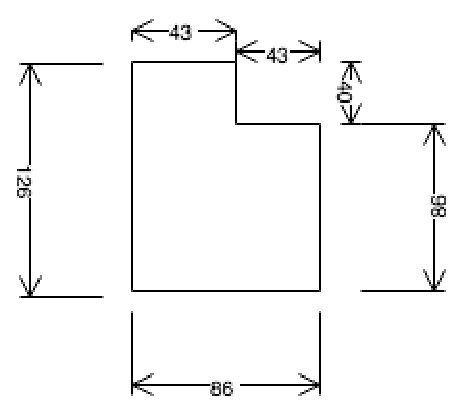
\includegraphics[scale=1.3]{figuras/map1.eps}
	\caption[Primeiro Cenário de Teste]{Mapa utilizado durante primeiro cenário de teste.}
	\label{img:map1}
\end{figure}

\subsection{Cenário de Teste 1}

Os resultados obtidos com o cenário estão dispostos na Tabela \ref{tab:cen1}. Deve-se atentar que o exemplo 3 possui um agravante, o
robô teve sua roda direita presa na parede enquanto se locomovia. Desse modo, o robô se perdeu e teve que se encontrar novamente, se comportando
da maneira esperada em um caso básico de "sequestro do robô".

Este cenário faz referência a variação da quantidade de partículas.

\begin{table}[H]
  \centering
  \caption{Resultados obtidos - Cenário 1}
  \label{tab:cen1}
  \begin{tabular}{|c|c|c|c|c|c|}
  \hline
  \textbf{Exemplo} & \textbf{Partículas} & \textbf{Rotação} & \textbf{Deslocamento} & \textbf{Movimentos} & \textbf{Precisão}\\ \hline
  1                & 200                   & 100             & 100                    & 9                & Ótima \\ \hline
  2                & 400                   & 100             & 100                    & 10                & Boa \\ \hline
  3                & 500                   & 100             & 100                    & 21                & Mediana \\ \hline
  4                & 100                   & 100             & 100                    & 5                & Mediana \\ \hline
  5                & 150                   & 100             & 100                    & 3                & Ótima \\ \hline
  \end{tabular}
\end{table}


\subsection{Cenário de Teste 2}

Os resultados obtidos com o cenário estão dispostos na Tabela \ref{tab:cen2}. Este cenário faz referência a variação da velocidade de
rotação do robô.

\begin{table}[H]
  \centering
  \caption{Resultados obtidos - Cenário 2}
  \label{tab:cen2}
  \begin{tabular}{|c|c|c|c|c|c|}
  \hline
  \textbf{Exemplo} & \textbf{Partículas} & \textbf{Rotação} & \textbf{Deslocamento} & \textbf{Movimentos} & \textbf{Precisão}\\ \hline
  1                & 150                   & 10             & 100                    & 7                & Boa \\ \hline
  2                & 150                   & 30             & 100                    & 6                & Ótima \\ \hline
  3                & 150                   & 50             & 100                    & 3                & Boa \\ \hline
  4                & 150                   & 70             & 100                    & 3                & Mediana \\ \hline
  5                & 150                   & 90             & 100                    & 8                & Mediana \\ \hline
  \end{tabular}
\end{table}


\subsection{Cenário de Teste 3}

Os resultados obtidos com o cenário estão dispostos na Tabela \ref{tab:cen3}. Este cenário faz referência a variação da velocidade de
deslocamento do robô, em unidades do diâmetro das rodas por segundo. Fixou-se a quantidade de partículas em 150, de acordo com os resultados
obtidos nos cenários anteriores, assim como a velocidade de rotação em 30 graus por segundo.

\begin{table}[H]
  \centering
  \caption{Resultados obtidos - Cenário 3}
  \label{tab:cen3}
  \begin{tabular}{|c|c|c|c|c|c|}
  \hline
  \textbf{Exemplo} & \textbf{Partículas} & \textbf{Rotação} & \textbf{Deslocamento} & \textbf{Movimentos} & \textbf{Precisão}\\ \hline
  1                & 150                   & 30             & 2                    & 4                & Baixa\\ \hline
  2                & 150                   & 30             & 5                    & 6                & Mediana\\ \hline
  3                & 150                   & 30             & 10                    & 3                & Baixa\\ \hline
  4                & 150                   & 30             & 15                    & 6                & Boa \\ \hline
  5                & 150                   & 30             & 30                    & 5                & Mediana\\ \hline
  \end{tabular}
\end{table}

\subsection{Cenário de Teste 4}

Os resultados obtidos com o cenário estão dispostos na Tabela \ref{tab:cen4}. Este cenário faz referência a análise da solução
utilizando a configuração que obteve os melhores resultados nos cenários anteriores, ou seja:

\begin{itemize}
  \item \textbf{Partículas:} 150
  \item \textbf{Rotação:} 30
  \item \textbf{Deslocamento:} 15
\end{itemize}

O objetivo principal deste cenário é verificar a variabilidade dos resultados utilizando configuração fixa durante os exemplos.

\begin{table}[H]
  \centering
  \caption{Resultados obtidos - Cenário 4}
  \label{tab:cen4}
  \begin{tabular}{|c|c|c|c|c|c|}
  \hline
  \textbf{Exemplo} & \textbf{Partículas} & \textbf{Rotação} & \textbf{Deslocamento} & \textbf{Movimentos} & \textbf{Precisão}\\ \hline
  1                & 150                   & 30             & 15                    & 8                & Mediana \\ \hline
  2                & 150                   & 30             & 15                    & 4                & Baixa \\ \hline
  3                & 150                   & 30             & 15                    & 5                & Baixíssima \\ \hline
  4                & 150                   & 30             & 15                    & 7                & Mediana \\ \hline
  5                & 150                   & 30             & 15                    & 8                & Boa \\ \hline
  \end{tabular}
\end{table}
